
% This LaTeX was auto-generated from an M-file by MATLAB.
% To make changes, update the M-file and republish this document.

\documentclass{article}
\usepackage{graphicx}
\usepackage{color}

\sloppy
\definecolor{lightgray}{gray}{0.5}
\setlength{\parindent}{0pt}

\begin{document}

    
    

\section*{Naive Bayes classifier for binary fisheriris digits}

\begin{verbatim}
loadData('fisheriris')
% meas: [150x4 double]
% species: [150x1 cell]
fisheriris.raw = [meas ones(150,1)];
fisheriris.raw(51:100,5) = 2;
fisheriris.raw(101:150,5) = 3;

%Randomize Data
fisheriris.random = fisheriris.raw(randperm(size(fisheriris.raw,1)),:);

%Categorize
fisheriris.train_labels = fisheriris.random(1:100,5);
fisheriris.test_labels = fisheriris.random(101:150,5);
fisheriris.train_images = fisheriris.random(1:100,1:4);
fisheriris.test_images = fisheriris.random(101:150,1:4);

% reshape to be size Ntrain*Ndims
ytrain = fisheriris.train_labels;
ytest = fisheriris.test_labels;
Xtrain = reshape(fisheriris.train_images, [1*4 100])';
Xtest = reshape(fisheriris.test_images, [1*4 50])';

% Binarize
for c=1:10
    digit=c-1;
    ndx = find(ytrain==digit);
    mu = mean(Xtrain(ndx,:));
    Xtrain(ndx,:) = Xtrain(ndx,:) > repmat(mu,length(ndx),1);
    ndx = find(ytest==digit);
    Xtest(ndx,:) = Xtest(ndx,:) > repmat(mu,length(ndx),1);
end
% save space
clear mnist
Xtrain = logical(Xtrain);
Xtest = logical(Xtest);


%trainSize = [1000 5000 10000 30000 60000];
trainSize = [100 50]; % 10000];
Ntest = 50;
for trial=1:length(trainSize)
    Ntrain = trainSize(trial);
    model = naiveBayesFit(Xtrain(1:Ntrain,:), ytrain(1:Ntrain)+1);
    yhat = naiveBayesPredict(model, Xtest(1:Ntest,:))-1; % 0..9
    ndxError = find(yhat ~= ytest(1:Ntest));
    nerr = length(ndxError)
    errorRate(trial) = nerr/Ntest %#ok
end
classConf = classConfMat(ytest(1:Ntest), yhat)/Ntest;

figure;
plot(trainSize, errorRate, 'o-', 'linewidth', 3, 'markersize', 10)
xlabel('training set size')
ylabel('test error rate')
title('Naive bayes on binarized fisheriris digits')
printPmtkFigure('mnistNaiveBayesErrVsN')


C=setdiag(classConf,0);figure;imagesc(C);colorbar
set(gca,'yticklabel',0:9)
set(gca,'xtick',1:10,'xticklabel',0:9)
title('class confusion matrix')


for j=1:min(2,length(ndxError))
    i=ndxError(j);
    figure;
    img = reshape(Xtest(i,:), [1 4]);
    imagesc(img);
    colormap(gray)
    title(sprintf('testcase %d, ytrue = %d, yhat = %d', i, ytest(i), yhat(i)));

end
\end{verbatim}

        \color{lightgray} \begin{verbatim}nerr =
    29
errorRate =
    0.5800    0.7000
nerr =
    35
errorRate =
    0.5800    0.7000
\end{verbatim} \color{black}
    
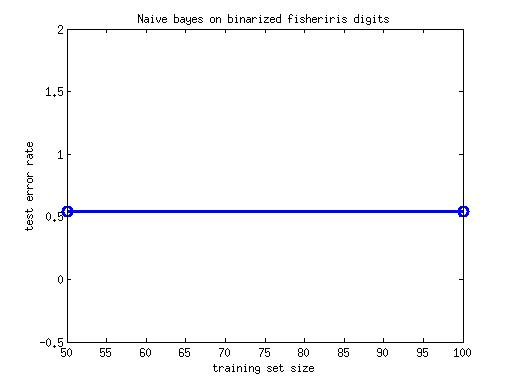
\includegraphics [width=4in]{HW2_MachineLearning_01.eps}

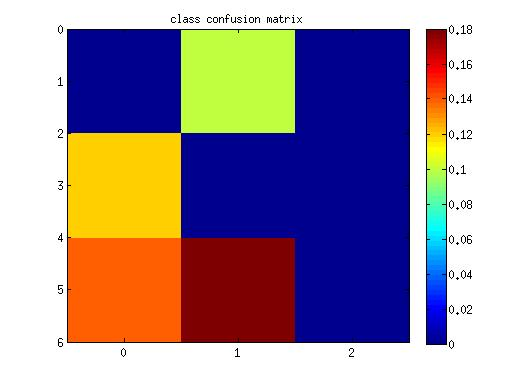
\includegraphics [width=4in]{HW2_MachineLearning_02.eps}

\includegraphics [width=4in]{HW2_MachineLearning_03.eps}

\includegraphics [width=4in]{HW2_MachineLearning_04.eps}



\end{document}
    
